\documentclass{beamer}
% Try the class options [notes], [notes=only], [trans], [handout],
% [red], [compress], [draft] and see what happens!

% \usepackage{definitions}
\usepackage[british]{babel}
\usepackage{color, soul}
\usepackage{tikz}

%% tikz tricks
% \tikzset{onslide/.code args={<#1>#2}{%
%   \only<#1>{\pgfkeysalso{#2}} 
% }}

\pdfinfo{
        /Title (cim)
        /Creator (LaTeX)
        /Producer (pdflatex)
        /Author (szerzo)
        /CreationDate (datum)
	/Subject (tema)
}


\mode<article> % only for the article version
{
  \usepackage{fullpage}
  \usepackage{hyperref}
}
\mode<presentation>
{
  \usetheme[left,width=0.65in,height=0.55in]{Kolozsvar}
  \setbeamercovered{transparent}
  \setbeamertemplate{navigation symbols}{}
  \setbeamertemplate{footline}%
     {\vspace*{-1.4em}\hspace*{0.66in}\textbf{\insertframenumber/\inserttotalframenumber}\newline\vspace*{0.4em}}
		\setbeamerfont{block title}{size=\larger} % RELSIZE -- html-sizes 
		\usefonttheme{professionalfonts}
		\setbeamercolor{math text}{fg=green!30!red!30!brown}
		\setbeamercolor{normal text in math text}{parent=math text}
}

\setbeamercovered{dynamic}

% The following info should normally be given in you main file:
\title[IoT in 5G Era]{IoT in 5G Era}

%
\author{Hunor Ördög, Norbert-Raymond Pap, István-Lehel Balázs}
%
\institute[UBB Cluj-Napoca]{
  Department of Mathematics and Informatics\\
  Babe{\c{s}}--Bolyai University, Cluj-Napoca}
%
\date{2024 December}


\begin{document}

\frame{\maketitle}

\mode<presentation>
{
  % \begin{frame}
  %   \frametitle{Talk structure}
  % \tableofcontents
  % \end{frame} 

  % \AtBeginSection[]
  {
      \begin{frame}<beamer>{Contents}
        % \tableofcontents[currentsection,currentsubsection,hideothersubsections]
        \tableofcontents
      \end{frame}
    }
}

%%%%%%%%%%%%%%%%%%%%%%%%%%%%%%%%%%%%%%%%%%%%%%%%%%%%%%%%%%%%%%%%%%%%%%

% \section[Brand changes - 28 oct 2024]{Brand changes - 28 oct 2024}

% \begin{frame}{Brand changes - 28 oct 2024}
  % \hspace*{2.3em}
  % \includegraphics[scale=0.25]{fig/sonar-rebrand-1.jpg}
% \end{frame}


% \section[Introduction]{Introduction}

% \begin{frame}{What is Sonar?}
%   \begin{itemize}
%     \item Tool for \textbf{code quality} and \textbf{security} throughout the development lifecycle.
%     \vspace*{0.75em}
%     \item Catch \textbf{bugs}, \textbf{vulnerabilities}, and \textbf{design issues} 
%     (Duplicated code, Large methods, Inconsistent naming).
%     \vspace*{0.75em}
%     \item Improve \textbf{maintainability}, \textbf{readability}, and \textbf{security}.
%   \end{itemize}
% \end{frame}


\section[Private 5G Network]{Private 5G Network}

\begin{frame}{Private 5G Network Classification}
  \hspace*{0.6em}
  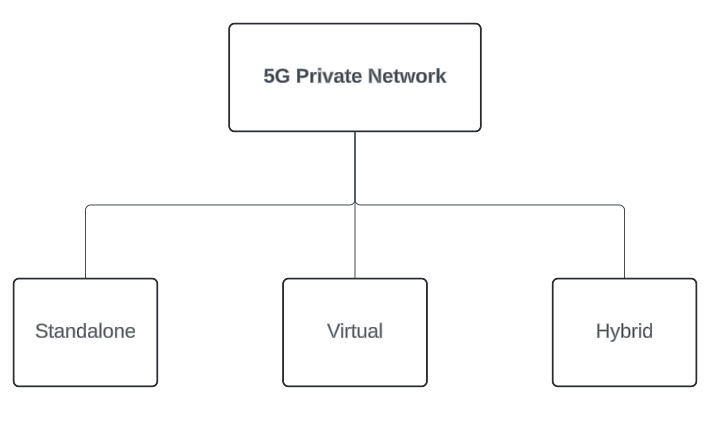
\includegraphics[scale=0.6]{fig/5gprivate.png}
\end{frame}


\begin{frame}{Standalone Private Network}
  \vspace*{1.6em}
  \begin{itemize}
    \item Purchased from an operator.
    \vspace*{0.75em}
    \item Mantained by customer.
    \vspace*{0.75em}
    \item Example: Airport - isolated network deployed physically at the airport's vicinity.
  \end{itemize}
\end{frame}

\begin{frame}{Virtual Private Network}
  \vspace*{1.6em}
  \begin{itemize}
    \item Virtualization on public 5G networks.
    \vspace*{0.75em}
    \item Logically private, but physically using the public network.
    \vspace*{0.75em}
    \item Example: Smart cars - virtual private network for operations.
  \end{itemize}
\end{frame}

\begin{frame}{Hybrid Private Network}
  \vspace*{1.6em}
  \begin{itemize}
    \item Combination of standalone and virtual.
    \vspace*{0.75em}
    \item Example: Manufacturing plant - enabling better distribution of functionalities along with broad coverage, high capacity, and cost-efficiency.
  \end{itemize}
\end{frame}

\section[Network exposure]{Network exposure}


\begin{frame}{What is Network Exposure in 5G?}
  \vspace*{1.6em}
  \begin{itemize}
    \item Allow customers and partners to access network services and capabilities via  easy-to-use APIs.
    \item Enables customers and partners to use network resources based on the needs of their applications.
    \item Crucial for IoT applications.
    \item Access is controlled by strict policies to ensure data integrity and protection.
  \end{itemize}
\end{frame}


\begin{frame}{Ericson's IoT experiment}
  \vspace*{1.3em}
  \begin{itemize}
    \item A remote controlled drone connected to 5G network is used to inspect a tower.
    \item The application uses APIs to trigger an exposure server on a 5G core network.
    \item API\#1 triggers exposure server to connect to the drone, authenticate, send it towards the tower.
    \item Inspection camera doesn't need to send high-quality video. 
  \end{itemize}
\end{frame}

\begin{frame}{Ericson's IoT experiment}
  \vspace*{1.6em}
  \begin{itemize}
    \item When the drone gets closer the application sends to API\#2 to increase bandwidth.
    \item Before reaching the tower the application sends to API\#3 to add URLLC slice for remote control, increase the quality of video.
    \item After the control the application sends to API\#4 to erase URLLC slice and lower the quality.
  \end{itemize}
\end{frame}

\begin{frame}{Experiment summary}
  \hspace*{0.4em}
  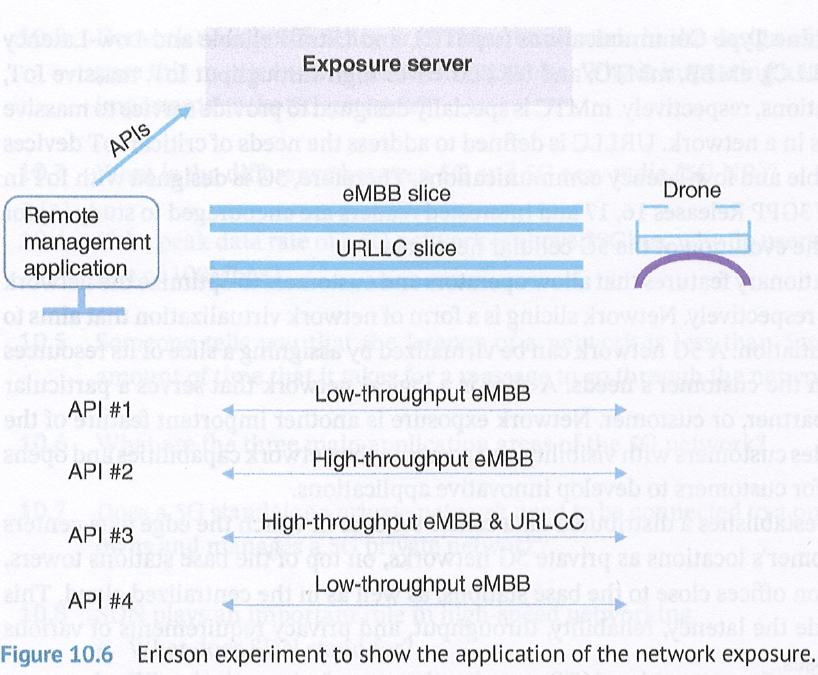
\includegraphics[scale=0.52]{fig/exposure-exp.png}
\end{frame}


\section[Fixed Wireless Access]{Fixed Wireless Access}


\begin{frame}{Fixed Wireless Access (FWA)}
  \vspace*{1.6em}
  \begin{itemize}
    \item Some locations don't have acces to wired internet connection.
    \vspace*{0.75em}
    \item 5G FWA can be used to provide internet access cost-effectively.
    \vspace*{0.75em}
    \item This way IoT devices can also get good internet access on remote places.
  \end{itemize}
\end{frame}


\section[Summary]{Summary}


\begin{frame}{Summary}
  \begin{itemize}
    \item enhanced Mobile BroadBand (eMBB).
    \vspace*{0.75em}
    \item massive Machine Type Communications (mMTC).
    \vspace*{0.75em}
    \item Ultra-Reliable and Low-Latency Communications (URLLC).
    \vspace*{0.75em}
    \item Network Slicing, Network Virtualization.
    \vspace*{0.75em}
    \item Private Networks, FWA.
  \end{itemize}
\end{frame}



\section[Exercises]{Exercises}


\begin{frame}{Exercises}
  \textbf{Question:} Compare 4G and 5G networks based on latency, speed, capacity, bandwidth and energy consumption.
\end{frame}

\begin{frame}{Exercises}
  \textbf{4G Network:}
  \begin{itemize}
    \item Latency: 30-50 ms
    \item Speeds: 1 Gbps (stationary), 100 Mbps (mobile)
    \item Capacity: 2,000 devices/km\(^2\)
    \item Bandwidth: Sub-6 GHz, limited in dense areas
    \item Energy: Higher per bit
  \end{itemize}
  \vspace{0.5cm}
  \textbf{5G Network:}
  \begin{itemize}
    \item Latency: As low as 1 ms
    \item Speeds: Up to 20 Gbps
    \item Capacity: 1 million devices/km\(^2\)
    \item Bandwidth: Sub-6 GHz + mmWave (24 GHz+)
    \item Energy: Lower per bit
  \end{itemize}
\end{frame}

\begin{frame}{Exercises}
  \textbf{Question:} 5G Supports 24-100Ghz frequency range, called FR2. What is the rande of wavelengths of FR2?
\end{frame}


\begin{frame}{Exercises}
  \textbf{Question:} 5G Supports 24-100Ghz frequency range, called FR2. What is the rande of wavelengths of FR2?
  \vspace*{0.75em}
  \begin{itemize}
    \item \textbf{Formula:} \(wavelength = \frac{c}{f}\), where \(c = 3 \times 10^8 \, \text{m/s}\)
    \item \textbf{For 24 GHz:}
    \[
    f = 24 \, \text{GHz} = 24 \times 10^9 \, \text{Hz}
    \]
    \[
      wavelength = \frac{3 \times 10^8 \, \text{m/s}}{24 \times 10^9 \, \text{Hz}} = 0.0125 \, \text{m} = 1.25 \, \text{cm}
    \]
    \item \textbf{For 100 GHz:}
    \[
    f = 100 \, \text{GHz} = 100 \times 10^9 \, \text{Hz}
    \]
    \[
      wavelength = \frac{3 \times 10^8 \, \text{m/s}}{100 \times 10^9 \, \text{Hz}} = 0.003 \, \text{m} = 3 \, \text{mm}
    \]
  \end{itemize}
\end{frame}

\begin{frame}{Exercises}
  \textbf{Question:} If the peak rate of 5G network is above 20Gbps, why do users only experience a data rate of 100Mbps?
\end{frame}


\begin{frame}{Exercises}
  \textbf{Question:} If the peak rate of 5G network is above 20Gbps, why do users only experience a data rate of 100Mbps?
  \vspace*{0.75em}
  \begin{itemize}
    \item It is not possible for the network to allow the user to transmit continuously using max number of possible data rate at all times.
    \item It has to share the resources between all the users in a cell.
    \item The data rate a user can experience depends on the location of the device in the cell, number of devices in the cell, their traffic pattern.
  \end{itemize}
\end{frame}


\begin{frame}{Exercises}
  \textbf{Question:} Does a 5G standalone private network need to be connected to a public 5G network? Who owns and manages it?
\end{frame}

\begin{frame}{Exercises}
  \textbf{Question:} Does a 5G standalone private network need to be connected to a public 5G network? Who owns and manages it?
  \vspace*{0.75em}
  \begin{itemize}
    \item No, it is isolated from the public network. 
    \item Standalone private networks are the ones purchased from the provider, and managed by the customer.
  \end{itemize}
\end{frame}


\end{document}
